\documentclass[12pt,a4paper]{report}
\usepackage[left=2.5cm,right=2.5cm,top=3cm,bottom=3cm]{geometry}
\usepackage{fancyhdr}
\usepackage{etoolbox}
\usepackage{titlesec}
\usepackage{titling} % para personalizar el título
\usepackage{amssymb}
\usepackage{amsmath}
\usepackage{graphicx}
\usepackage{ulem}
\usepackage{cancel}
\usepackage{enumitem}
\usepackage{lmodern}

\pagestyle{fancy}
\fancyhf{} 
\fancyhead[L]{UTN-FRC}
\fancyhead[C]{ASyS}
\fancyhead[R]{2R3}
\renewcommand{\headrulewidth}{0.4pt}
\fancyfoot[C]{\vfill\thepage}

\patchcmd{\chapter}{\thispagestyle{plain}}{\thispagestyle{fancy}}{}{}

\renewcommand{\chaptername}{Ejercicio}

\titleformat{\chapter}[display]
  {\normalfont\bfseries}{\chaptertitlename\ \thechapter}{15pt}{}
\titlespacing*{\chapter}{0pt}{-30pt}{-30pt}

\setlength{\headheight}{15pt}

\DeclareMathSizes{15}{13}{8}{8}

\setlength{\parskip}{6pt}

\title{%
  \fontsize{25}{0}\selectfont Universidad Tecnológica Nacional \\
  \fontsize{22}{30}\selectfont Analisis de Señales y Sistemas \\
  \fontsize{20}{25}\selectfont Trabajo Practico 2
}
\author{
Alejo Agustin Lopez Demichelis\\
Franco Palombo\\
Ignacio Gil\\
Jesus Agustin Frigerio\\
Laureano Valentin Reinoso\\
Luciano Tomas Cortesini Perez\\
Matias Gabriel Moran\\
Leonardo Ramos\\
}
\date{19 / 08 / 2024}

\begin{document}
\maketitle

\chapter{}%ejercicio 1

\textbf{Movimiento Rectilíneo Uniformemente Variado (MRUV) - Caída libre}

\begin{itemize}
  \item Un primer cuerpo de masa $m_1$ se deja caer (verticalmente) desde una posición inicial $y_0 > 0$.

  \item Un segundo cuerpo de igual masa que el primero, se deja caer (verticalmente) desde una posición inicial 
     $\frac{1}{2} y_0$, es decir, a mitad de camino del primer cuerpo.

\end{itemize}

Teniendo como punto de referencia el "suelo", responder las siguientes consignas:

\begin{enumerate}[label=\alph*)]
  \item Realizar un gráfico que represente la situación de los dos cuerpos en caída libre, sus respectivos vectores 
    de velocidad y posición.

  \item Determinar las ecuaciones de cinemáticas para la posición $y_1(t)$ y $y_2(t)$ en función del tiempo para cada
    uno de los cuerpos, respectivamente. \textbf{Reflexionar:} ¿las funciones $y_1, y_2$ pueden interpretarse como 
    señales de variable de tiempo continuo? ¿Las masas de los cuerpos intervienen en la descripción de las funciones
    $y_1(t),y_2(t)$?

  \item Calcular el tiempo de vuelo (total) $T$ del primer cuerpo, en función de $y_0$. Similarmente, calcular el 
    tiempo de vuelo $\tau$ del segundo cuerpo. ¿Qué relación aritmética encuentra entre los dos tiempos $T$ y $\tau$?
    ¿Se puede obtener $y_2$ como un escalonado en el tiempo de la señal $y_1$?

  \item Calcular el tiempo $t_0$ que le toma al primer cuerpo estar en la posición $\frac{1}{2} y_0$. ¿Qué relación 
    aritmética encuentra entre $t_0$ y $\tau$? ¿Se puede obtener $y_2$ como una traslación temporal de la señal $y_1$?

  \item \textbf{Reflexionar:} ¿Tiene sentido físico evaluar la señal $y_1$ en tiempos $t > T$? Similarmente, ¿tiene 
    sentido físico evaluar la señal $y_2$ en tiempos $t > \tau$? En caso afirmativo, ¿cuál es la interpretación
    física? Y en caso negativo, emplear alguna herramienta para redefinir las señales $y_1, y_2$, de tal forma que la 
    información provista por el futuro sea nula. Por otra parte, ¿tiene sentido físico evaluar a las señales $y_1,
    y_2$ en tiempos negativos $t < 0$? En caso afirmativo, ¿qué representa? Y en caso negativo, emplear alguna 
    herramienta para redefinir las señales $y_1, y_2$ de tal forma que la información provista por el pasado sea nula.

  \item Teniendo en cuenta las señales redefinidas del inciso anterior $y_1, y_2$ (pasado y futuro de la señal son
    nulos) verificar si estas cumplen (o no) cada una de las siguientes propiedades: Periódica, Energía finita, 
    Potencia finita, causal, acotada.

\end{enumerate}

\textbf{Movimiento Armónico Simple (MAS) - Masa/Resorte}

Considerar un sistema conformado por una Masa $m$, atada a la derecha de un resorte con constante elástica $\kappa$, 
dispuesto en forma horizontal y sujetado en el extremo izquierdo. Teniendo como punto de referencia la posición de
equilibrio, máxima amplitud $A > 0$ y despreciando los efectos de la fricción, responde las siguientes consignas:

\begin{enumerate}[label=\alph*)]
  \item Realizar un gráfico que represente el sistema y sus respectivos vectores de fuerza.

  \item Determinar la ecuación de cinemática para la posición $x(t)$ en función del tiempo. \textbf{Reflexionar:} ¿la
    función $x$ puede interpretarse como una señal de variable de tiempo continua?

  \item Es de conocimiento general que la función posición $x(t)$ se puede determinar en función del $seno$ o del 
    coseno. Determinar la transformación temporal sobre la señal, la cual permite pasar de la formulación $seno$ a la 
    formulación $coseno$.

  \item Verificar si la señal $x(t)$ cumple (o no) cada una de las siguientes propiedades: Periódica, Energía finita,
    Potencia finita, causal, acotada.
\end{enumerate}

\chapter{}%ejercicio 2
Considerar las siguientes señales proporcionadas por un rectificador de onda completa y $1/2$ onda respectivamente:
\textbf{Señal Sinusoidal rectificada de onda completa}, $x_1(t)$ determinada por el gráfico:

% Incluir aquí el gráfico de la señal sinusoidal rectificada de onda completa

\textbf{Señal Sinusoidal rectificada de media onda}, $x_2(t)$ determinada por el gráfico:

% Incluir aquí el gráfico de la señal sinusoidal rectificada de media onda

\begin{enumerate}[label=\alph*)]
  \item Calcular el periodo fundamental $T_0$ de las señales $x_1, x_2$. ¿Las señales tienen energía finita? Calcular
    la energía relativa a un intervalo con longitud un periodo fundamental $T_0$.

  \item Teniendo en cuenta que la potencia media de una señal se define como

  $$P_1 = \lim_{r \to \infty} \frac{1}{2r} \int_{-r}^{r} |x(t)|^2 \, dt$$

  \begin{itemize}
    \item Demostrar la siguiente igualdad, válida para señales periódicas en donde la potencia media relativa a un
      intervalo con longitud un periodo fundamental $T_0$ coincide con la potencia media, es decir:

     $$P_1 = \frac{1}{T_0} \int_{t_0}^{t_0 + T_0} |x(t)|^2 \, dt$$

    \item Calcular la potencia media $P_1$ de la señal $x_1$ y similarmente, $P_2$ de la señal $x_2$.

  \end{itemize}

  \item Considerar el conjunto de señales básicas

  $$\{\psi_n(t) = \cos(n\omega t) \mid n \geq 0\} \cup \{\varphi_n(t) = \sin(n\omega t) \mid n \geq 1\}$$

  \begin{itemize}
    \item Calcular la energía relativa a un intervalo con longitud un periodo fundamental $T_0$ y el periodo $T_n$
      de cada señal del conjunto, y luego, demostrar que (dos a dos) forman un conjunto de señales ortogonales más no
      ortonormales.

      \textbf{Reflexión:} ¿si los periodos $T_n$ de cada señal del conjunto básico son distintos, por qué la suma 
      (finita/infinita) es periódica? ¿Por qué se restringe el dominio del tiempo en un intervalo del tipo 
      $t_0 \leq t \leq t_0 + T_0$, si las señales básicas están bien definidas en todo el eje temporal?

   \item Obtener la representación de las señales $x_1, x_2$ como una combinación lineal de las señales básicas, 
     esto es, calcular coeficientes $(a_n, b_n)$ en $\mathbb{R}$ tales que:

     $$x_1 = \sum_{n=0}^{\infty} a_n \psi_n + \sum_{n=1}^{\infty} b_n \varphi_n$$
     Similarmente para la señal $x_2$.

   \item Truncar la suma infinita del inciso anterior en $n = 5$ y hacer un gráfico comparativo entre la señal 
     original $x_1$ y su aproximación trigonométrica. Similarmente para la señal $x_2$.

  \end{itemize}

  \item Considerar el conjunto de señales básicas

  $$\{\phi_n(t) = e^{jn\omega t} \mid n \in \mathbb{Z}\}$$

  Notar que la siguiente relación entre las señales con parámetro negativo y el conjugado:

  $$\phi(-n) = \phi_n^*, \forall n \geq 0$$

  \begin{itemize}

    \item Calcular la energía relativa a un intervalo con longitud un periodo fundamental $T_0$ y el periodo $T_n$ de
      cada señal del conjunto, y luego, demostrar que (dos a dos) forman un conjunto de señales ortogonales más no
      ortonormales.\newline
      \textbf{Reflexión:} ¿si los periodos $T_n$ de cada señal del conjunto básico son distintos, por qué la suma
      (finita/infinita) es periódica? ¿Por qué se restringe el dominio del tiempo en un intervalo del tipo 
      $t_0 \leq t \leq t_0 + T_0$, si las señales básicas están bien definidas en todo el eje temporal?

    \item Obtener la representación de las señales $x_1, x_2$ como una combinación lineal de las señales básicas, esto 
      es, obtener coeficientes $C_n$ en $\mathbb{C}$ tales que

      $$x_1 = \sum_{-\infty < n < \infty} C_n \phi_n =
      \sum_{n=1}^{\infty} C_{-n} \phi_n^* + C_0 \phi_0 + \sum_{n=1}^{\infty} C_n \phi_n$$

      Similarmente para la señal $x_2$.

    \item Considerar $|n| \leq 5$ y realizar el espectro de frecuencias de ambas señales en fase, esto es, graficar los 
      pares ordenados

      $$\{(n, \text{Arg}(C_n)) \mid -5 \leq n \leq 5\}$$
      correspondientes a cada señal $x_1, x_2$.

      \item Considerar $|n| \leq 5$ y realizar el espectro de frecuencias de ambas señales en módulo, esto es, graficar 
        los pares ordenados

      $$\{(n, |C_n|) \mid -5 \leq n \leq 5\}$$

      correspondientes a cada señal $x_1, x_2$.\newline

    \item Calcular una aproximación a las potencias medias $P_1, P_2$, por medio de la relación de Parseval con los 
      espectros de frecuencia de ambas señales en módulo (usar la información de los incisos anteriores) y discriminar 
      el aporte de las componentes (CC, AC).

      \textbf{Reflexionar:} ¿Qué ventajas/desventajas encuentra entre el método directo para calcular la potencia media 
      $P_1, P_2$ de las señales $x_1, x_2$ en la variable de tiempo $t$ y el método que se deriva de la relación de 
      Parseval, en donde los cálculos se realizan en la variable $n \in \mathbb{Z}$?

  \end{itemize}

  \item Comparar los espectros obtenidos para cada una de las señales $x_1, x_2$, evaluar y proponer las 
    características sobresalientes de ambos espectros.
\end{enumerate}

\chapter{}%ejercicio 3

Considerar $G_T(t) = \mu_{(t + \frac{T}{2})} - \mu_{(t - \frac{T}{2})}$ una señal pulso rectangular con duración finita 
$T$ y amplitud unitaria.

\begin{enumerate}[label=\alph*)]
  \item Realizar el gráfico de las señales $x_1 = G_1(t)$ y $x_2 = G_{0.1}(t)$, luego, calcular la energía $E_1$ de 
    $x_1$, y similarmente $E_2$ de $x_2$.

  \item Obtener la transformada de Fourier $F_1(\omega) = \mathcal{F}\{x_1\}$ y similarmente $F_2(\omega) = 
    \mathcal{F}\{x_2\}$. Reflexionar: ¿En qué variable están definidas las funciones $F_1, F_2$? 
    ¿Qué representa la variable $\omega$ y qué diferencia tiene con la variable $t$? 
    ¿Las funciones $F_1, F_2$ resultan periódicas?
  
  \begin {itemize}
    \item Graficar el espectro de frecuencia en fase para $F_1, F_2$, esto es, graficar los pares ordenados
    $$\{(\omega, \text{Arg}(F)) \mid \omega \in \mathbb{R}\}$$

    Para cada una de las funciones $F_1, F_2$.\newline
    \textbf{Reflexionar:} ¿El espectro de frecuencia en fase es discreto o continuo? ¿El gráfico admite una simetría
    par, impar o ninguna?
    \item Graficar el espectro de frecuencia en módulo para $F_1, F_2$, esto es, graficar los pares ordenados
    $$\{(\omega, |F|) \mid \omega \in \mathbb{R}\}$$

    Para cada una de las funciones $F_1, F_2$.\newline
    \textbf{Reflexionar:} ¿El espectro de frecuencia en módulo es discreto o continuo? ¿El gráfico admite una 
    simetría par, impar o ninguna?
    \item Graficar la densidad espectral para $F_1, F_2$, esto es, graficar los pares ordenados
    $$\{(\omega, |F|^2) \mid \omega \in \mathbb{R}\}$$

    Para cada una de las funciones $F_1$, $F_2$.\newline
    \textbf{Reflexionar:} ¿La densidad espectral es discreta o continua? ¿El gráfico admite una simetría par, impar o
    ninguna?

    \item Calcular la energía $E_1, E_2$ haciendo uso de la relación de Parseval.
    Reflexionar: ¿Qué ventajas/desventajas encuentra entre el método directo para calcular la energía $E_1, E_2$ de
    las señales $x_1, x_2$ en la variable de tiempo $t$ y el método que se deriva de la relación de Parseval, en
    donde los cálculos se realizan en la variable $\omega$?

  \end{itemize}

  \item Comparar los espectros obtenidos para cada una de las señales $x_1, x_2$, evaluar y proponer las 
    características sobresalientes de ambos espectros.

\end{enumerate}

\chapter{}%ejercicio 4

  \textbf{Circuito Eléctrico RC:} circuito eléctrico correspondiente a un sistema de 1° orden y su ecuación
  característica:
  $$v(t) = R\cdot i(t) + \frac{1}{C} \cdot \int_{0}^{t} i(\tau) d\tau$$

  \noindent
  \begin{figure}[h]
    \centering
    \begin{minipage}[h]{0.5\textwidth}
      \centering
      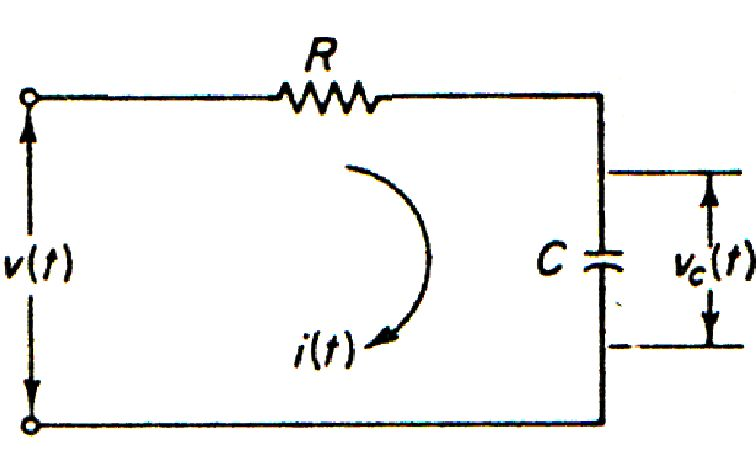
\includegraphics[width=1\textwidth]{./images/Ej4.1.jpg}
      \textit{Circuito RC}
    \end{minipage}
  \end{figure}

  \begin{enumerate}[label=\alph*)]
    \item Obtener una representación del circuito con Ecuaciones Diferenciales de primer orden y coeficientes
      constantes, y con ello, definir un Sistema en tiempo continuo con entrada $x(t) = v(t)$ y salida $y(t) = i(t)$.
      Luego, hacer un diagrama de bloques de la E.D; exponiendo los integradores que la conforma.

    \item Teniendo en cuenta el siguiente resultado matemático, obtener una descripción explicita
      de la respuesta $y(t)$ del sistema obtenido en el inciso anterior:
      \begin{itemize}
        \item Sean $\alpha, \beta_0, \beta_1 \in R$ constantes; $y(t), x(t)$ funciones con variable de tiempo continuo,
          las cuales verifican la ecuación diferencial de primer orden con coeficientes constantes:

          $$y_t'+\alpha y_t = \beta_1 x_t' + \beta_0 x_t$$

          Entonces, una Solución General explicita de la Ecuación Diferencial es

          $$y_t = \beta_1 x_t + (y_0 - \beta_1 x_0) e^{-\alpha t} + (\beta_0 - \alpha \beta_1) \int_{0}^{t} x(\tau)
          e^{-\alpha(t - \tau)} d\tau$$

          donde $y_0 = y(0), x_0 = x(0)$ son Condiciones Iniciales arbitrarias
        \end{itemize}

    \item Usando la descripción explicita de la salida del Sistema $y_t = S_1{x_t}$ (CI arbitrarias) del inciso
      anterior, calcular la respuesta a cada una de las siguientes señales:

      $$x_0(t) = 0, \hspace{0.5cm}x_1(t) = \mu_t, \hspace{0.5cm}x_2(t) = \mu(t - t_0), \hspace{0.5cm}x_3(t) =
      \mu_t - \mu(t - t_0), \hspace{0.5cm}x_4(t) = t$$

      \textbf{Reflexionar:} ¿La señal $y_0$ es completamente nula? ¿Las señales $y_3, y' = y_1 - y_2$ (iguales o
      distintas)? ¿es suficiente para garantizar la Linealidad del sistema? ¿Las señales $y_1, y_2$ son iguales? ¿es
      suficiente para garantizar la Inv. Tiempo del sistema?.

    \item Usando la descripción explicita de la salida del Sistema $y_t = S_1{x_t}$ (CI arbitrarias), demostrar si el
      Sistema $S1$ es (o no): Lineal, Homogéneo e Invariante en el Tiempo.

    \item Demostrar que el sistema anterior en reposo gana propiedades, esto es, definir $y_t = S_2{x_t}$ con C.I. 
      nulas $y_0 = x_0 = 0$, y clasificar el sistema S2 (Aditivo, Homogéneo, Inv. Tiempo).

    \item Refinar aun más el sistemas, exijamos C.I nulas y respuesta causal (se elimine el pasado), esto es, definir 
      $y_t = S_3{x_t} = S_2{x_t} \mu_t$. Demostrar que el sistema S3 es LIT (Lineal e Inv. Tiempo). Sintetizar sus 
      respuestas es una tabla de doble entrada:

      \begin{table}[h!]
        \centering
        \begin{tabular}{|c|c|c|c|}
          \hline
          \textbf{Entrada $x_t$} & \textbf{Salida $y_t = S_3{x_t}$} & \textbf{Salida $y_t = x_t * h_t$} & \textbf{Comparar}\\
          \hline
          $\delta_t$ & $h_t = ??$ & &\\
          \hline
          $\mu_t$ & & &\\
          \hline
          $\mu_{t-1}$ & & &\\
          \hline
          $\mu_t - \mu_{t-1}$ & & &\\
          \hline
          $t$ & & &\\
          \hline
          $t\mu_{t}$ & & &\\
          \hline
          $e^{2t}$ & & &\\
          \hline
          $e^{2t}\mu_{-t}$ & & &\\
          \hline

        \end{tabular}
      \end{table}
      \textbf{Reflexionar:} En general, ¿cualquier sistema $S$ admite una descripción del tipo $S{x} = y = x * h$?
      ¿Cuales son los requerimientos para que esto suceda? ¿El dominio de señales de entrada del sistema linealizado
      $S_3{x}$, es igual al dominio del sistema $x * h$?


  \end{enumerate}

\end{document}
